
% ----------------------------------------------------------------------
%  Set the document class
% ----------------------------------------------------------------------
\documentclass[11pt,a4paper,twoside]{article}

% ----------------------------------------------------------------------
% Define external packages, language, margins, fonts and new commands
% ----------------------------------------------------------------------
%\input{preamble} 
\usepackage[utf8]{inputenc}   % <<<<< Linux
\usepackage[english]{babel} % <<<<< English
\usepackage{notoccite}
\usepackage[skip=0.5\baselineskip]{caption}
\hyphenation{GTKWave}
\usepackage{listings}
\usepackage[all]{nowidow}
\usepackage{amsmath}

%blind text
\usepackage{lipsum}

\usepackage{graphicx}
\graphicspath{{./}{../../figlib/}{../mat/}{../sim/}}
\def\FontLn{% 16 pt normal
  \usefont{T1}{phv}{m}{n}\fontsize{16pt}{16pt}\selectfont}
\def\FontLb{% 16 pt bold
  \usefont{T1}{phv}{b}{n}\fontsize{16pt}{16pt}\selectfont}
\def\FontMn{% 14 pt normal
  \usefont{T1}{phv}{m}{n}\fontsize{14pt}{14pt}\selectfont}
\def\FontMb{% 14 pt bold
  \usefont{T1}{phv}{b}{n}\fontsize{14pt}{14pt}\selectfont}
\def\FontSn{% 12 pt normal
  \usefont{T1}{phv}{m}{n}\fontsize{12pt}{12pt}\selectfont}

% Use Arial font as default
%
\renewcommand{\rmdefault}{phv}
\renewcommand{\sfdefault}{phv}
\usepackage{geometry}	
\geometry{verbose,tmargin=2.5cm,bmargin=2.5cm,lmargin=2.5cm,rmargin=2.5cm}

%\usepackage{setspace}
%\renewcommand{\baselinestretch}{1.5}

\usepackage[pdftex]{hyperref} % enhance documents that are to be
                              % output as HTML and PDF
\hypersetup{colorlinks,       % color text of links and anchors,
                              % eliminates borders around links
%            linkcolor=red,    % color for normal internal links
            linkcolor=black,  % color for normal internal links
            anchorcolor=black,% color for anchor text
%            citecolor=green,  % color for bibliographical citations
            citecolor=black,  % color for bibliographical citations
%            filecolor=magenta,% color for URLs which open local files
            filecolor=black,  % color for URLs which open local files
%            menucolor=red,    % color for Acrobat menu items
            menucolor=black,  % color for Acrobat menu items
%            pagecolor=red,    % color for links to other pages
            pagecolor=black,  % color for links to other pages
%            urlcolor=cyan,    % color for linked URLs
            urlcolor=black,   % color for linked URLs
	          bookmarks=true,         % create PDF bookmarks
	          bookmarksopen=false,    % don't expand bookmarks
	          bookmarksnumbered=true, % number bookmarks
	          pdftitle={report},
            pdfauthor={Andre C. Marta},
%            pdfsubject={Thesis Title},
%            pdfkeywords={Thesis Keywords},
            pdfstartview=FitV,
            pdfdisplaydoctitle=true}

\usepackage[numbers,sort&compress]{natbib} % <<<<< References in numbered list [1],[2],...
\usepackage{subcaption} 
\usepackage{mdframed}
\usepackage{gensymb}

%%%%%%%%%%%%%%%%%%%%%%%%%%%%%%%%%%%%%%%%%%%%%%%%%%%%%%%%%%%%%%%%%%%%%%%%
%     Begin Document                                                   %
%%%%%%%%%%%%%%%%%%%%%%%%%%%%%%%%%%%%%%%%%%%%%%%%%%%%%%%%%%%%%%%%%%%%%%%%


\begin{document}

% Set plain page style (no headers, footer with centered page number)
\pagestyle{plain}

% Set roman numbering (i,ii,...) before the start of chapters
%\pagenumbering{roman}

% ----------------------------------------------------------------------
%  Cover page
% ----------------------------------------------------------------------
%%%%%%%%%%%%%%%%%%%%%%%%%%%%%%%%%%%%%%%%%%%%%%%%%%%%%%%%%%%%%%%%%%%%%%%%
%                                                                      %
%     File: Thesis_FrontCover.tex                                      %
%     Tex Master: Thesis.tex                                           %
%                                                                      %
%     Author: Andre C. Marta                                           %
%     Last modified :  2 Jul 2015                                      %
%                                                                      %
%%%%%%%%%%%%%%%%%%%%%%%%%%%%%%%%%%%%%%%%%%%%%%%%%%%%%%%%%%%%%%%%%%%%%%%%

\thispagestyle {empty}

% IST Logo - Signature A
% parameters: bb=llx lly urx ury (bounding box), width=h_length, height=v_length, angle=angle, scale=factor, clip=true/false, draft=true/false. 
\includegraphics[bb=9.5cm 11cm 0cm 0cm,scale=0.29]{IST_A_CMYK_POS}

\begin{center}
%
% Figure (Image or plot)
\vspace{1.0cm}
% height = 50 mm
%\includegraphics[height=50mm]{Figures/Airbus_A350.jpg}

% Title, author and degree
\vspace{1cm}
{\FontLb Circuit Theory and Electronics Fundamentals} \\ % <<<<< EDIT TITLE
\vspace{1cm}
{\FontSn Instituto Superior Técnico, University of Lisbon} \\ % <<<<< EDIT COURSE
\vspace{1cm}
{\FontSn Laboratory Report: Lab Assignment T1} \\
\vspace{1cm}
{\FontSn March, 2021} \\ % <<<<< EDIT DATE (corresponds to date of oral examination)
%
\end{center}



% ----------------------------------------------------------------------
% Dedication page (optional)
% ----------------------------------------------------------------------
%\input{dedication} 
%\cleardoublepage

% ----------------------------------------------------------------------
%  Acknowledgments (optional)
% ----------------------------------------------------------------------
%\input{acknowledgements}
%\cleardoublepage

% ----------------------------------------------------------------------
%  Abstract (both in English and Portuguese)
% ----------------------------------------------------------------------
%\input{resumo} 
%\cleardoublepage

%\input{abstract} 

% ----------------------------------------------------------------------
%  Table of contents, list of tables, list of figures and nomenclature
% ----------------------------------------------------------------------

% Table of contents
%
\tableofcontents

% List of tables
%\addcontentsline{toc}{section}{\listtablename}
%\listoftables
%\cleardoublepage 

% List of figures
%\addcontentsline{toc}{section}{\listfigurename}
%\listoffigures
%\cleardoublepage 

% Set arabic numbering (1,2,...) after preface
%
%\setcounter{page}{1}
%\pagenumbering{arabic}

% ----------------------------------------------------------------------
%  Body
% ----------------------------------------------------------------------

\clearpage

\vspace{-0.25cm}
\section{Introduction}
\label{sec:introduction}

The aim of this laboratory assignment is to build an audio amplifier with the goal
of maximizing the gain and bandwidth and minimizing the total cost and the value of lower cut-off frequency.
The circuit designed has two distinct parts: the gain stage and the output stage as shown in figure \ref{fig:circuito}.

\begin{figure}[h] \centering
    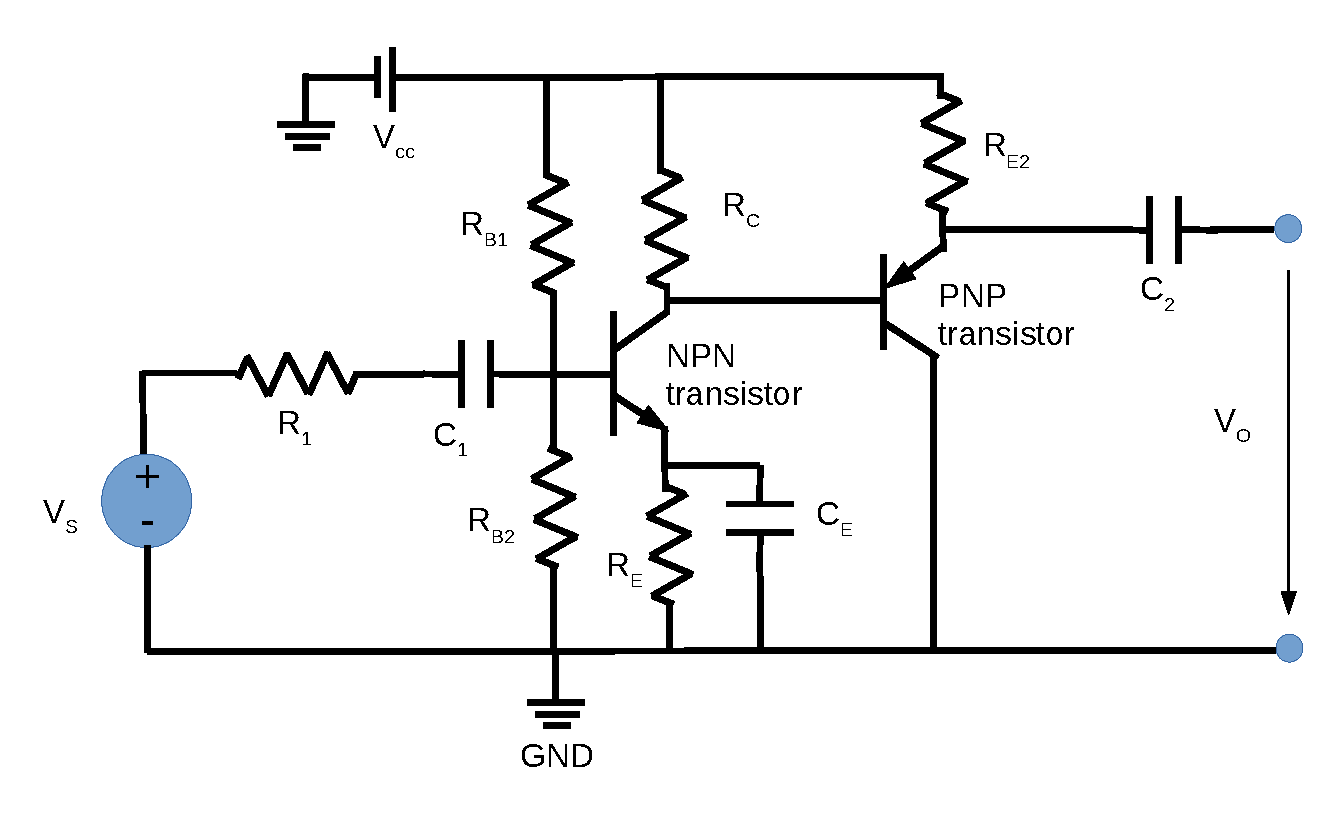
\includegraphics[scale=0.7]{lab4_principal.pdf}
    \caption{Circuit analysed.}
    \label{fig:circuito}
\end{figure}

The input ($V_{s}$) is a sinusoidal signal with a maximum amplitude of 10mV with an internal impendance of 100 $\Omega$, represented by $R_{in}$.
On the other end of the circuit we can find an 8 $\Omega$ speaker. Additionally, the circuit is supplied
by a 12V DC source, $V_{cc}$, that garantees that the transistor operates in its forward-active region (Base Biasing).

The gain stage mentioned, which is connected to the input signal, is formed by a single stage common-emitter amplifier
with degeneration that uses a NPN transistor. Furthermore, there is a bias circuit and a bypass capacitor which
functions will be discussed later in the report.
Moving on to the output stage, it was used a common collector amplifier but this time a PNP transistor was used.
This stage is basically responsible for lowering the output impendace that comes from the previous stage,
so that the values are appropriate for the speaker.

Now we will talk about the goal of the coupling capacitors ($C_{1}$ and $C_{2}$), bypass capacitors ($C_{3}$) and the effect of the resistance $R_{C}$.


Starting with the $C_{1}$ and $C_{2}$, they are low impendance coupling capacitors and DC blocking capacitors whose reactance at the signal frequency is designed to be negligible.
The AC coupling through capacitors is used to inject AC input signal and extract output signal without disturbing the Q-point (steady-state voltage or current at a specified terminal of an active device with no input signal applied.)
For this reason they have a direct impact on the lower and upper 3dB cut off frequencies and therefore the bandwidth of the network.

***

At low frequencies the reactance of coupling capacitor C2 is relatively high and hence very small part of the signal will pass from the amplifier stage to the load.
At high frequencies the reactance of coupling capacitor C2 is very small and it behaves as a short circuit. This increases the loading effect of the amplifier stage and serves to reduce the voltage gain.
At mid frequencies the voltage gain of the amplifier is constant. The effect of the coupling capacitor C2 in this frequency range is such as to maintain a constant voltage gain. Thus, as the frequency increases in this range, the reactance of C2 decreases, which tends to increase the gain.
If it is not used, then the amplified AC signal following through $R_{E}$ will cause a voltage drop across it, thereby dropping the output voltage.

***

$C_{3}$ is a bypass capacitor that provides a low impendace path for the AC current from emitter to ground,
thereby removing $R_{E}$ (required for good Q-point stability) from the circuit when AC signals are considered which garantees that the resistor will not affect the gain.

Finally, não sei o que dizer em relação a esta resistência.


In Section~\ref{sec:analysis}, a theoretical analysis of the circuit is performed, followed by an simulation in \ref{sec:simulation}
with the goal of comparing and understand better the behaviour of this circuit.

%\begin{figure}[h] \centering
%    \includegraphics[scale=0.6]{}
%    \caption{Circuit analysed.}
%    \label{fig:rc}
%\end{figure}

%\begin{figure}[h] \centering
%    \includegraphics[scale=0.4]{}
%    \caption{Positive half.}
%    \label{fig:rc2}
%\end{figure}

%\begin{figure}[h] \centering
%    \includegraphics[scale=0.4]{}
%    \caption{Negative half.}
%    \label{fig:rc3}
%\end{figure}

%\begin{figure}[h] \centering
%    \includegraphics[scale=0.75]{}
%    \caption{Wave rectified.}
%    \label{fig:rc4}
%\end{figure}

%\begin{figure}[h] \centering
%    \includegraphics[scale=0.75]{}
%    \caption{Wave rectified, with filter.}
%    \label{fig:rc5}
%\end{figure}




\newpage
\section{Theoretical Analysis}
\label{sec:analysis}

In this section, the circuit shown in figure \ref{fig:rc} is analysed
theoretically.

\newpage









\section{Simulation Analysis}
\label{sec:simulation}

We decided to, once again, put the circuit's scheme down below, so as to make the interpretation of the following results easier (fig \ref{fig:op}).

\subsection{Operating Point Analysis}

Table~\ref{tab:op} shows the simulated operating point results for the circuit
under analysis. As can be seen, we obtained similar results to the ones calculated in the theoretical analysis section. This is proof that our theoretical analysis is, indeed, correct.
We noticed, however, that \emph{Octave} rounded the values of the circuit's parameters ($R_{1}, ..., R_{7}, V_{a}, I_{d}, K_{b}, K_{c}$), whereas \emph{Ngspice} operated with the same precision as the one provided initially (no rounding).
As such, one could expect to find slightly different results. However, this did not prove to be the case. Another important thing to note is that we had to insert a fictitional
voltage source, with value $0\hspace{1mm}V$, in series with $R_{6}$ and $R_{7}$, in order to properly introduce the current $I_{c}$ in $V_{c}$'s calculation, in the current dependent
voltage source. This was due to \emph{Ngspice}'s limitations, though. Thus,
the value $V(6.5)$ in the table, which is equal to $V(6)$, like we required it to.

\begin{figure}[h] \centering
  \includegraphics[height=0.33\textheight]{t1_meshes.pdf}
  \caption{Circuit analysed.}
  \label{fig:op}
\end{figure}

\begin{table}[h]
  \centering
  \begin{tabular}{|l|r|}
    \hline    
    {\bf Name} & {\bf Value [A or V]} \\ \hline
    \input{../sim/op_tab}
  \end{tabular}
  \caption{Operating point. A variable preceded by @ is of type {\em current}
    and expressed in Ampere; other variables are of type {\it voltage} and expressed in
    Volt.}
  \label{tab:op}
\end{table}
\newpage





\section{Conclusion}
\label{sec:conclusion}

In this laboratory assignment, the objective of analysing the circuit presented
in figure \ref{fig:rc} has been achieved. The analysis was performed both theoretically
using the Octave maths tool and by circuit simulation using the Ngspice tool.
The simulation results matched the theoretical results precisely.
The reason for this perfect match is the fact that this is a
straightforward circuit containing only linear components, so the theoretical
and simulation models cannot differ. For more complex components, the
theoretical and simulation models could differ, but this is not the case in this
work. Even though the calculations were successful, we realised that we could have 
done a smarter choice of the reference node. For instance, if we had chosen node $4$ as the reference node, 
the equations would be a little simpler overall, since there would be more voltage values in the equations that would 
be equal to $0$. In addition, this choice of reference node would make us apply the supernode construct for the independent 
voltage source instead of the dependent one, making the equations easier once again, since there would be less diverging and 
converging currents to take into account.

\begin{thebibliography}{9}

    \bibitem{spicenotes}
    Phyllis R. Nelson.
    \textit{\href{https://www.cpp.edu/~prnelson/courses/ece220/220-spice-notes.pdf}{Introduction to \emph{spice} source files}}.
    \\\texttt{https://www.cpp.edu/ $\tilde{}$ prnelson/courses/ece220/220-spice-notes.pdf}


    \bibitem{octave}
    John W. Eaton, David Bateman, Søren Hauberg, Rik Wehbring.
    \textit{\href{https://octave.org/octave.pdf}{GNU Octave - Free Your Numbers}}.
    \\\texttt{https://octave.org/octave.pdf}

    \bibitem{libreoffice}
    LibreOffice Documentation Team.
    \textit{\href{https://documentation.libreoffice.org/assets/Uploads/Documentation/en/GS7.0/GS70-GettingStarted.pdf}{Getting Started Guide}}.
    \\\texttt{https://documentation.libreoffice.org/assets/Uploads/Documentation/en/
        GS7.0/GS70-GettingStarted.pdf}

    \bibitem{analysis}
    Mesh analysis and node analysis notes.
    \textit{\href{https://moodle.fct.unl.pt/pluginfile.php/167552/mod_resource/content/0/NotasTecnicas/Apontamento_tecnico_3_ebf.pdf}{Princípios fundamentais na análise de circuitos electrónicos}}.
    \\\texttt{https://moodle.fct.unl.pt/pluginfile.php/167552/mod$\_$resource/content/
        0/NotasTecnicas/Apontamento$\_$tecnico$\_$3$\_$ebf.pdf}

\end{thebibliography}

%\cleardoublepage

% ----------------------------------------------------------------------
%  Bibliography
% ----------------------------------------------------------------------
%\addcontentsline{toc}{section}{\bibname}
%\bibliographystyle{abbrvunsrtnat} % <<<<< SELECT IF USING REFERENCES BY NUMBER (CITATION ORDER)
%\bibliography{../../../BIBfile.bib}

% ----------------------------------------------------------------------
\end{document}
% ----------------------------------------------------------------------
